\documentclass[12pt, a4paper]{article}

\usepackage[english]{babel}
\usepackage{amsmath}
\usepackage{amssymb}
\usepackage{amsthm}
\usepackage{graphicx}
\usepackage{hyperref}
\usepackage{geometry}
\geometry{
	a4paper,
	left=20mm,
	right=20mm,
	top=25mm,
	bottom=25mm
}

\title{pestim - an R package to estimate population counts from aggregated mobile phone data}
\author{David Salgado\footnote{Department of Methodology and Development of Statistical Production, Statistics Spain (INE)}  and who else to add as author??}

\date{}



\begin{document}
\maketitle

\begin{abstract}
This package has been developed in the context of a European research project 
within the European Statistical System called ESSnet on Big Data.
It provides an implementation for a hierarchical model to combine both 
aggregated mobile phone data and external official (administrative or survey) 
data to produce estimates of population counts in each cell of a division of a territory using a Bayesian approach.
\end{abstract}


\section{Introduction}

\texttt{pestim} R package implements a hierarchical model to estimate the population counts of different territorial cells 
combining the information from aggregated 
mobile phone data and a population register or survey data, both at a given time instant and along a 
sequence of time periods. The theoretical model implemented by the \texttt{pestim} R package
follows the ecological sampling techniques to estimate population counts (see e.g. \cite{ManNacAlb15a} and 
\cite{RoyDor08a}) which are based on a bayesian approach. The complete methodology is described in \cite{methodology}.
The proposed model rests on two working assumptions:
\begin{itemize}
	\item Given that mobile phone data and official data operate at different 
time scales, we assume that there exists an initial time instant 
in which we can equate population figures from both sources.
	\item The mobility patterns of individuals do not depend on the mobile 
network operator which they are subscribed to.
\end{itemize}

The inference of the population counts from mobile phone data and official data is achieved in a two step process:
\begin{itemize}
	\item {at a given time instant $t_{0}$ both mobile phone and 
official data are used to infer the population counts in each territorial cell;}
	\item {at later moments, $t_{1}, t_{2},...$ the transition probabilities are inferred from mobile phone 
	data and are used to estimate the spatial and time evolution of the population.}
\end{itemize}


The package is structured on three layers of functions:
\begin{itemize}
	\item \textbf{Auxiliary functions}, providing computation of mathematical functions 
such as the ratio of two beta functions, the confluent hypergeometric function, 
an optimization routine for a concrete probability distribution, etc. 
Examples of these functions are \texttt{ratioBeta, kummer, Phi, modeLambda};
	\item \textbf{Distribution-related functions}, providing computation regarding
the generation of random deviates according to different probability distributions 
comprising both priors, posteriors, and the generation of parameter specifications 
for these distributions. Examples of these functions are 
\texttt{dtriang, rtriang, ptriang, qtriang, dlambda, rlambda, rmatProb, rN0, rNt, rNtcondN0, rg, rp, alphaPrior, genAlpha, genUV}.
\item \textbf{Estimation-related functions}, providing computation of estimates 
based upon the populations generated with the preceding functions. 
Examples of these functions are \texttt{postN0, postNt, postNtcondN0}.
\end{itemize}

\texttt{pestim} package is freely available under the \texttt{GPL3} and \texttt{EUPL} lincese 
at the following address: \url{https://github.com/MobilePhoneESSnetBigData/pestim}. 
It can be installed using \texttt{install\_github()} function from \texttt{devtools} package:
\begin{verbatim}
library(devtools)
install_github("MobilePhoneESSnetBigData/pestim")
\end{verbatim}

Since it contains \texttt{C++} code, the user need to install \texttt{Rtools} under Windows 
enviroment or to have a  \texttt{C++}  compiler under Linux or Mac OS X environments.

\section{The hierarchical model}\label{model}

In this section we will give a short description of the theoretical model 
underlaying the \texttt{pestim} R package for estimation of the population 
counts at a given time moment.

A first input of the model is 
$\mathbf{N}^{\textrm{MNO}}=(N_{1}^{\textrm{MNO}}, \dots, N_{I}^{\textrm{MNO}})^{T}$ which 
represents the population counts reported by the mobile network operator in 
each territorial cell $i\in\mathcal{I}=\{1,\dots,I\}$ (i.e. the aggregated mobile phone data). 
The second input of the model is the official population counts in each territorial cell denoted by 
$\mathbf{N}^{\textrm{REG}}=(N_{1}^{\textrm{REG}}, \dots, N_{I}^{\textrm{REG}})^{T}$. 
These official population counts could come from administrative data sources or from statistical surveys.
\texttt{pestim} implements a function to estimate the actual population 
counts $\mathbf{N}=(N_{1}, \dots, N_{I})^{T}$ combining both data sources. 
It also computes the posterior probability distribution 
$\mathbb{P}\left(\mathbf{N}|\mathbf{N}^{\textrm{MNO}};\mathbf{N}^{\textrm{REG}}\right)$ 
that can be used to assess the uncertainty in the output estimates.
This process can be represented schematically as shown in figure \ref{Tool}.

\begin{figure}
\makebox[\textwidth][c]{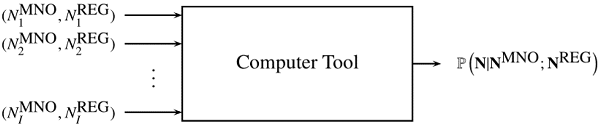
\includegraphics[width=0.7\textwidth]{Tool.png}}%
%%\centering
%%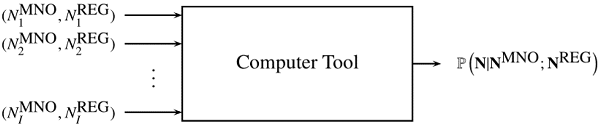
\includegraphics[width=1 \textwidth, natwidth=454, natheight=97]{Tool.png}
\caption{A diagram for the process of estimating population counts using mobile phone and official population data.}
\label{Tool}
\end{figure}


The main idea of the model is to emulate the ecological sampling setting in which 
the number of detected individuals in each cell follows a binomial distribution $Bin(N_{i}, p_{i})$ 
whose parameter $N_{i}$ is the target of the model and is assigned a weakly informative prior 
and the detection probability $p_{i}$ is also assigned a weakly informative prior based 
upon both data sources. In our case, if we have $N_{i}$ individuals in cell $i$ and we have an independent detection probability $p_{i}$ for each individual through the mobile telecommunication network, then we will detect $N_{i}^{\textrm{MNO}}$ individuals according to the aggregated mobile phone data naturally following a binomial distribution. $N_{i}$  can be modeled as Poisson random variables with independent parameters $\lambda_{i}$, variables which are pairwise independent, while $p_{i}$ are the proportions of individuals detected by the MNO at time $t_{0}$ in each cell $i$. It is importnt to note here that $p_{i}$ is not simply the market share of the MNO in cell $i$ but the actual proportion of individuals detected by the network. As an illustrative example, a call between a subscriber in a cell $i$ and a non-subscriber in another cell $j$ of a given MNO is certainly detected by the network in \emph{\textbf{both cells}}, thus potentially being part of the aggregated data $N_{i}^{\textrm{MNO}}$ and $N_{j}^{\textrm{MNO}}$. This example emphasizes the importance  of the knowledge of the preprocessing and aggregation procedures from microdata for the final result.


Thus, the model can be summarized as follows:

\begin{align}
N_{i}^{\textrm{MNO}}&\simeq\textrm{Bin}\left(N_{i}, p_{i}\right),\qquad N_{i}^{\textrm{MNO}}\perp N_{j}^{\textrm{MNO}},\quad i\neq j=1,\dots,I\\
N_{i}&\simeq\textrm{Po}\left(\lambda_{i}\right),\qquad N_{i}\perp N_{j},\quad i\neq j=1,\dots,I\nonumber\\
p_{i}&\simeq\textrm{Beta}\left(\alpha_{i},\beta_{i}\right),\qquad p_{i}\perp p_{j}\quad i\neq j=1,\dots,I\nonumber\\
\left(\alpha_{i}, \beta_{i}\right)&\simeq \frac{f_{1}(\frac{\alpha_{i}}{\alpha_{i}+\beta_{i}}; \mathbf{N}^{\textrm{REG}}, \mathbf{z})\cdot f_{2}(\alpha_{i}+\beta_{i}; \mathbf{N}^{\textrm{REG}}, \mathbf{z})}{\alpha_{i}+\beta_{i}}\quad
(\alpha_{i},\beta_{i})\perp(\alpha_{j},\beta_{j}),\quad i\neq j=1,\dots,I\nonumber\\
\lambda_{i}&\simeq f_{3}(\lambda_{i}; N_{i}^{\textrm{REG}}, \mathbf{z})\quad (\lambda_{i} > 0, \lambda_{i}\perp\lambda_{j}), \quad i=1,\dots,I.\nonumber
\end{align}



\begin{thebibliography}{99}

\bibitem{methodology}
~Deptartment of Methodology and Development of Statistical Production, Statistics Spain (INE), 
A hierarchical model to estimate population counts from
aggregated mobile phone data, January, 2018.

\bibitem{ManNacAlb15a}
~Manly, B.F.J., ~ Navarro Alberto, J.A., Introduction to ecological sampling,
CRC Press, 2015.

\bibitem{RoyDor08a}
~Royle, J.A., Dorazio, R.M., Hierarchical modeling and inference in ecology,
Academic Press, 2008.

\bibitem{BDA3}
~Gelman, A., ~Carlin, J.B., ~Stern, H.S., ~Dunson, D.B., ~Vehtari, A., ~Rubin, D.B., Bayesian Data Analysis (3rd ed), CRC Press, 2013

\bibitem{FlaSed95a}
~Flajolet, P., ~Sedgewick, R.,  Mellin transforms and asymptotics; Finite differences and Rice's integrals,
in  Theoretical Computer Science 144, pp. 101-124, 1995.

\bibitem{GraKnuPat96a}
Graham, R.L., ~Knuth, D.E., ~Patashnik, O., Concrete Mathematics (2nd ed.), 
Addison-Wesley, 1996.

\bibitem{Joh02a}
~Johnson, W.P., The curious history of Faà di Bruno's formula, in 
American Mathematical Monthly 109, pp. 217-234, March, 2002.

\bibitem{BroChu03a}
~Brown, J.W., ~Churchill, R.V., Complex variables and applications (7th ed.), 2003.

\bibitem{GraRyz07a}
~Gradshteyn, I.S., ~Ryzhik, I.M., Tables of Integrals, Series, and Products (7th ed.),
2007.

\bibitem{Dev86a}
~Devroye, L., Non-uniform random variable generation, Springer, 1986.

\bibitem{Q2016}
~De Meersman, F., ~Seynaeve, G., ~Debusschere, M., ~Lusyne, P., ~Dewitte, P., 
~Baeyens, Y., ~Wirthmann, A., ~Demunter, C., ~Reis, F., ~Reuter, H.I.,
Assessing the Quality of Mobile Phone Data as a Source of Statistics,
presented at Q2016 Conference, June, 2016.

\bibitem{WP5Del11}
~ESSnet on Big Data WP5, Current status of access to mobile phone data in the ESS, 2017.
 
\end{thebibliography}

\end{document}